% Carried over verbatim from monograph/main.tex (Study 1 record, 13 Sep 2026).
\chapter{Split protocols and structural leakage}\label{s1:ch:ch07_split_protocols_and_structural_leakage}

\section{Why four protocols are needed}

\begin{figure}[H]
\centering
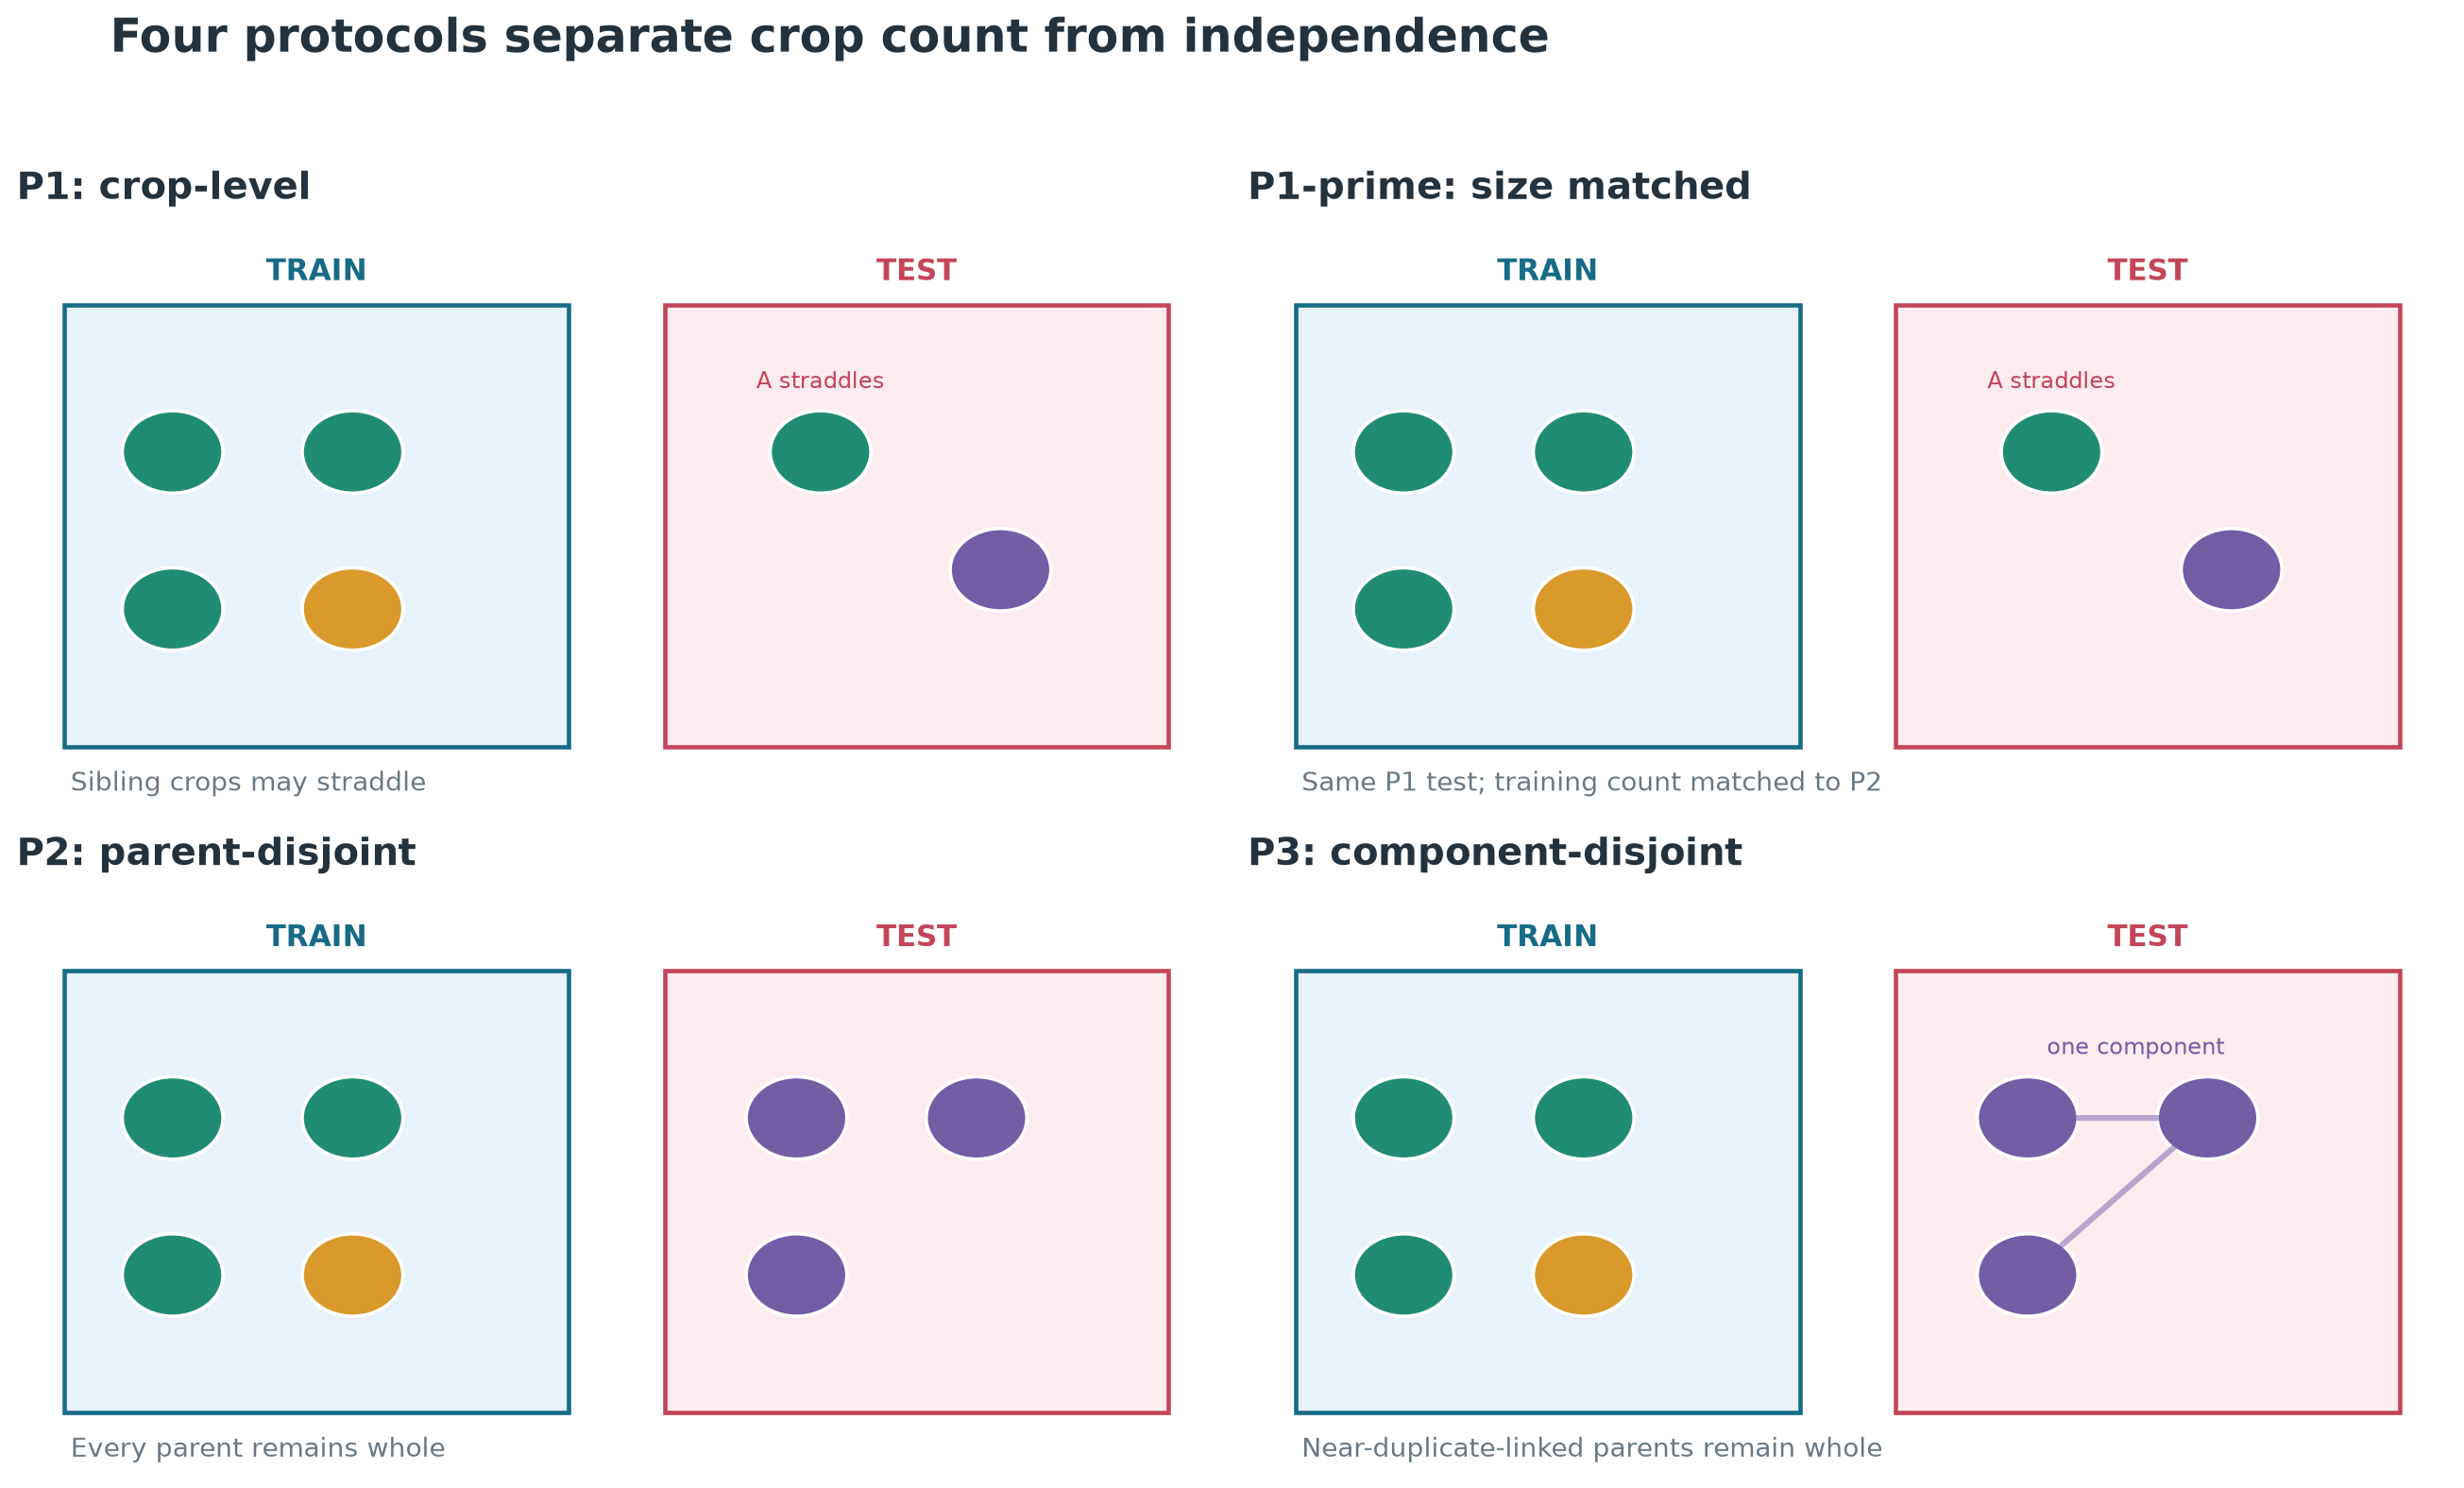
\includegraphics[width=\textwidth]{split_protocols.png}
\caption{The four protocols. P1 asks what common crop splitting shares. P1-prime holds its test set but matches the P2 training count. P2 groups exact parents. P3 groups whole near-duplicate-linked parent components.}
\label{s1:fig:protocols}
\end{figure}

All splits use an 80:20 target and the five fixed seeds. P1 is class-stratified at crop level. P1-prime retains P1's test observations and downsamples only its training observations to exactly the P2 training count, as closely class-balanced as integer counts permit. P2 uses group-aware allocation by exact parent. P3 repeats parent-disjoint allocation after cross-parent candidate links are collapsed into connected components.

On the frozen SIPaKMeD environment, P2 contains 3,239 train and 810 test crops for every seed. P1 already has exactly those counts, so P1-prime is identical to P1. This is not a redundant hidden comparison: it shows that the primary P1--P2 difference cannot be attributed to a larger P1 training set in this implementation.

\section{Analytic straddle probability}

For a parent with $k$ crops independently assigned to training with probability 0.8 and test with probability 0.2, the only non-straddling outcomes are ``all train'' and ``all test.'' Hence
\begin{align}
P(\text{no straddle}\mid k) &= 0.8^k+0.2^k,\\
P(\text{straddle}\mid k) &= 1-0.8^k-0.2^k.
\end{align}
For a dataset with parent crop counts $k_1,\dots,k_m$, the analytic expectation is
\begin{equation}
\bar{P}_{\text{straddle}}=\frac{1}{m}\sum_{j=1}^{m}\left(1-0.8^{k_j}-0.2^{k_j}\right).
\end{equation}

The exact class-stratified fixed-size splitter is not perfectly independent Bernoulli assignment. Therefore the analytic quantity is checked against a 10,000-allocation Monte Carlo interval generated with the actual count vector and allocation rule.

\begin{figure}[H]
\centering
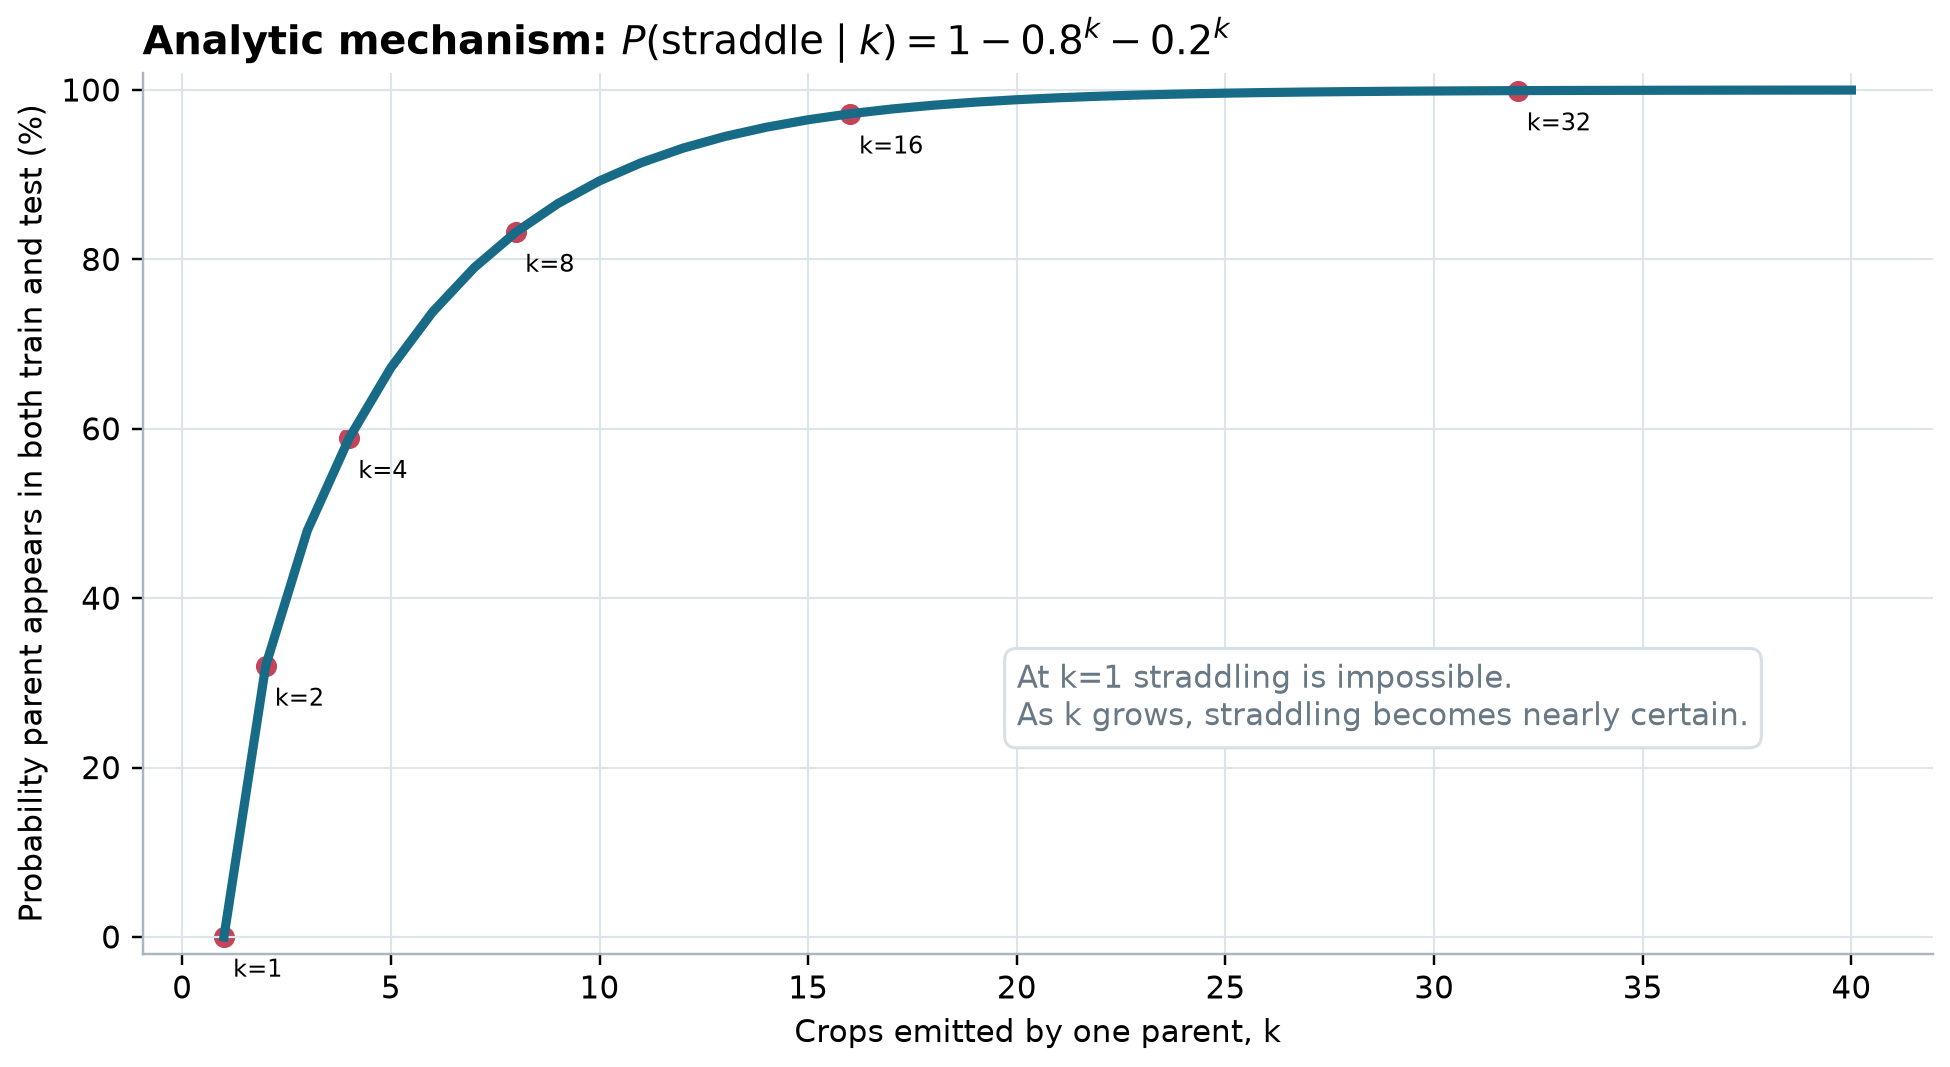
\includegraphics[width=0.87\textwidth]{straddle_probability.png}
\caption{The analytic mechanism. A one-crop parent cannot straddle; a high-multiplicity parent almost certainly straddles under independent 80:20 crop allocation.}
\label{s1:fig:straddle-curve}
\end{figure}

\section{Structural endpoints}

Let $G_{\mathrm{tr}}$ and $G_{\mathrm{te}}$ be training and test parent sets, and let $T$ be the test observations. The parent-straddle fraction and leaked-test-observation fraction are
\begin{equation}
L_p=\frac{|G_{\mathrm{tr}}\cap G_{\mathrm{te}}|}{|G|},\qquad
L_c=\frac{1}{|T|}\sum_{x\in T}\mathbf{1}\{g(x)\in G_{\mathrm{tr}}\}.
\end{equation}

\begin{table}[H]
\centering
\caption{Structural leakage. Stochastic values are mean $\pm$ sample SD over five seeds.}
\label{s1:tab:structural}
\resizebox{\textwidth}{!}{%
\begin{tabular}{lrrrrrr}
\toprule
Dataset & Crops & Parents & Analytic P1 straddle & Observed P1 straddle & P1 test with train parent & P2/P3 straddle \\
\midrule
SIPaKMeD & 4,049 & 966 & 44.83\% & 45.63$\pm$1.04\% & 92.62$\pm$0.40\% & 0.00$\pm$0.00\% \\
Cx22 & 1,320 & 514 & 33.93\% & 34.01$\pm$1.10\% & 85.23$\pm$3.51\% & 0.00$\pm$0.00\% \\
CRIC & 11,534 & 400 & 94.88\% & 94.35$\pm$1.10\% & 99.97$\pm$0.08\% & 0.00$\pm$0.00\% \\
Herlev & 917 & 917 & 0.00\% & 0.00$\pm$0.00\% & 0.00$\pm$0.00\% & 0.00$\pm$0.00\% \\
\bottomrule
\end{tabular}}
\end{table}

\begin{figure}[H]
\centering
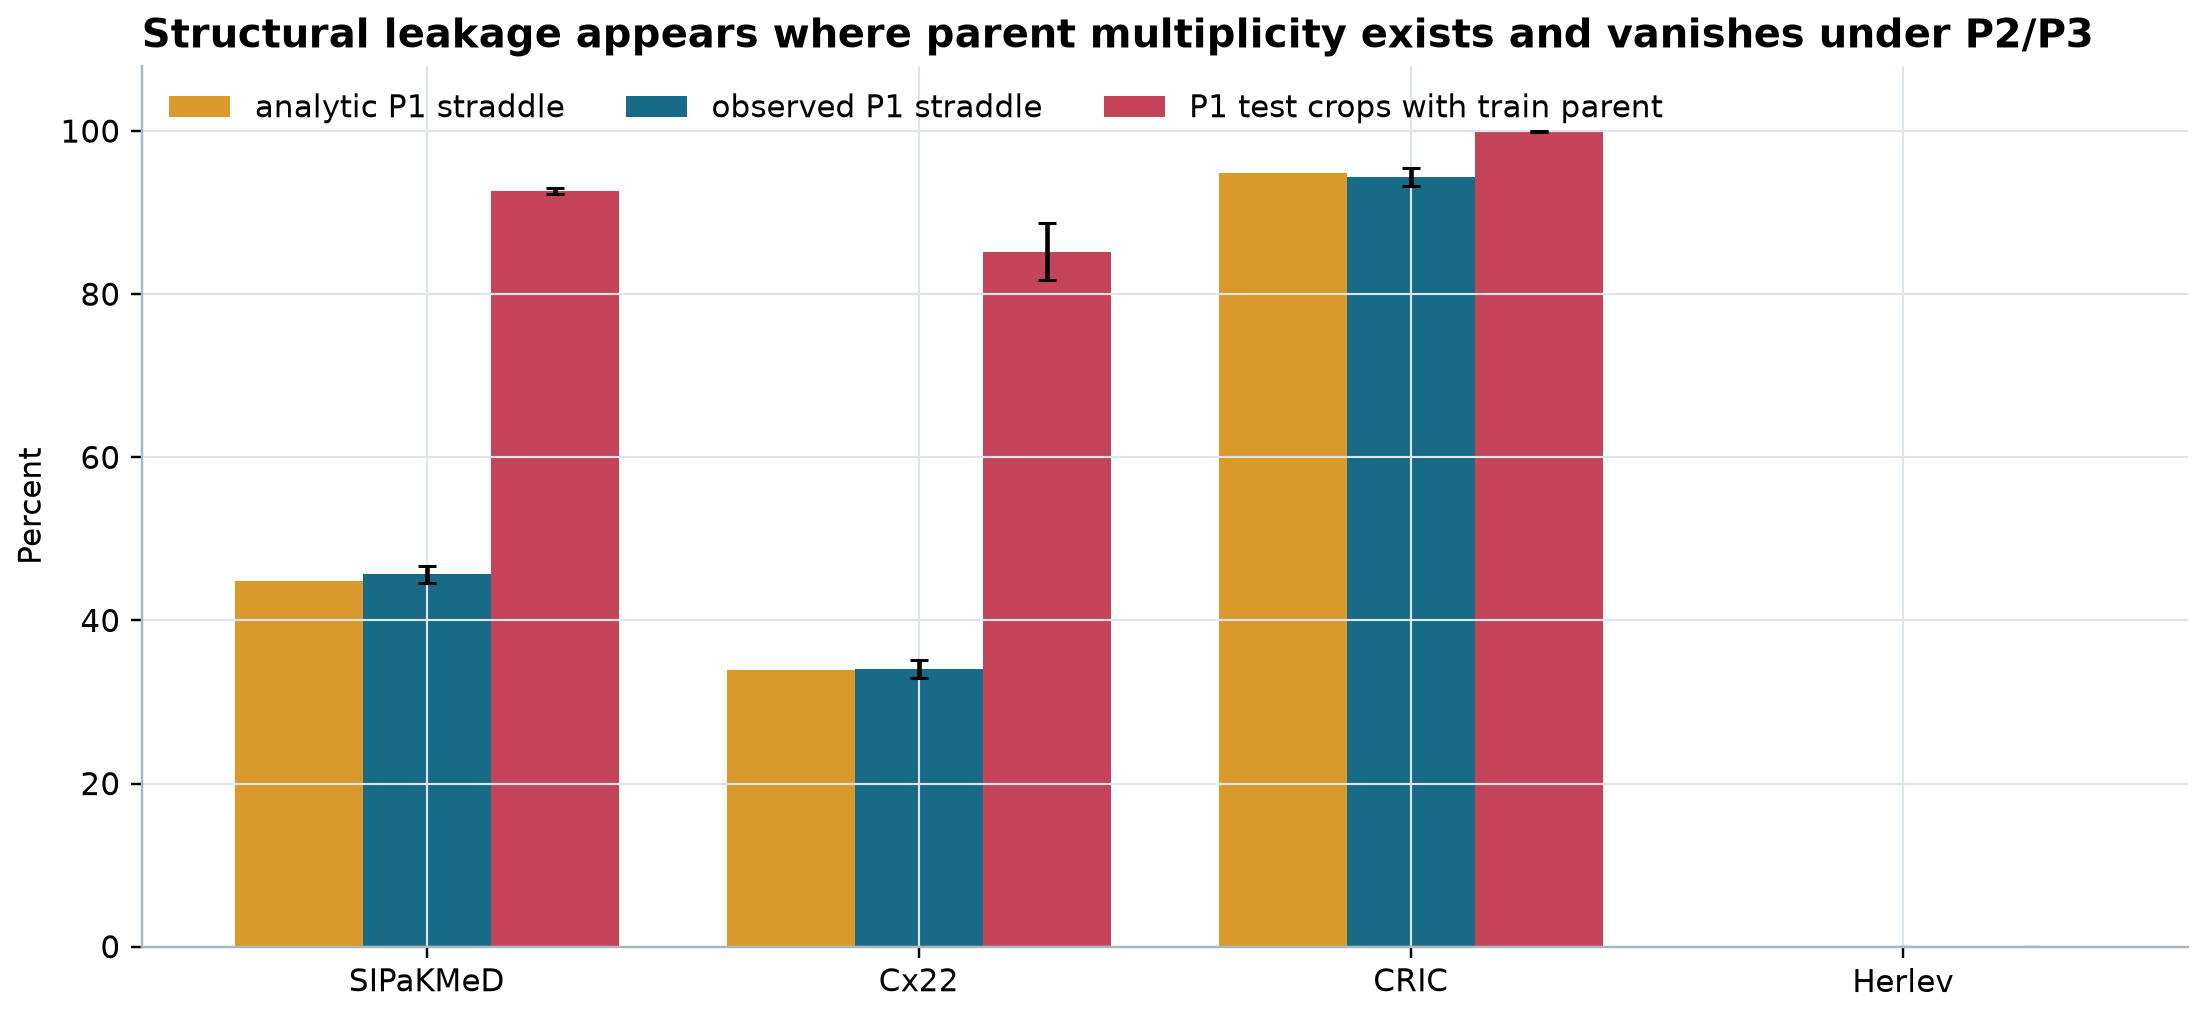
\includegraphics[width=\textwidth]{structural_results.png}
\caption{Analytic and observed leakage. P2 and P3 are omitted from the bars because both are exactly zero on all four datasets.}
\label{s1:fig:structural-results}
\end{figure}

\begin{figure}[H]
\centering
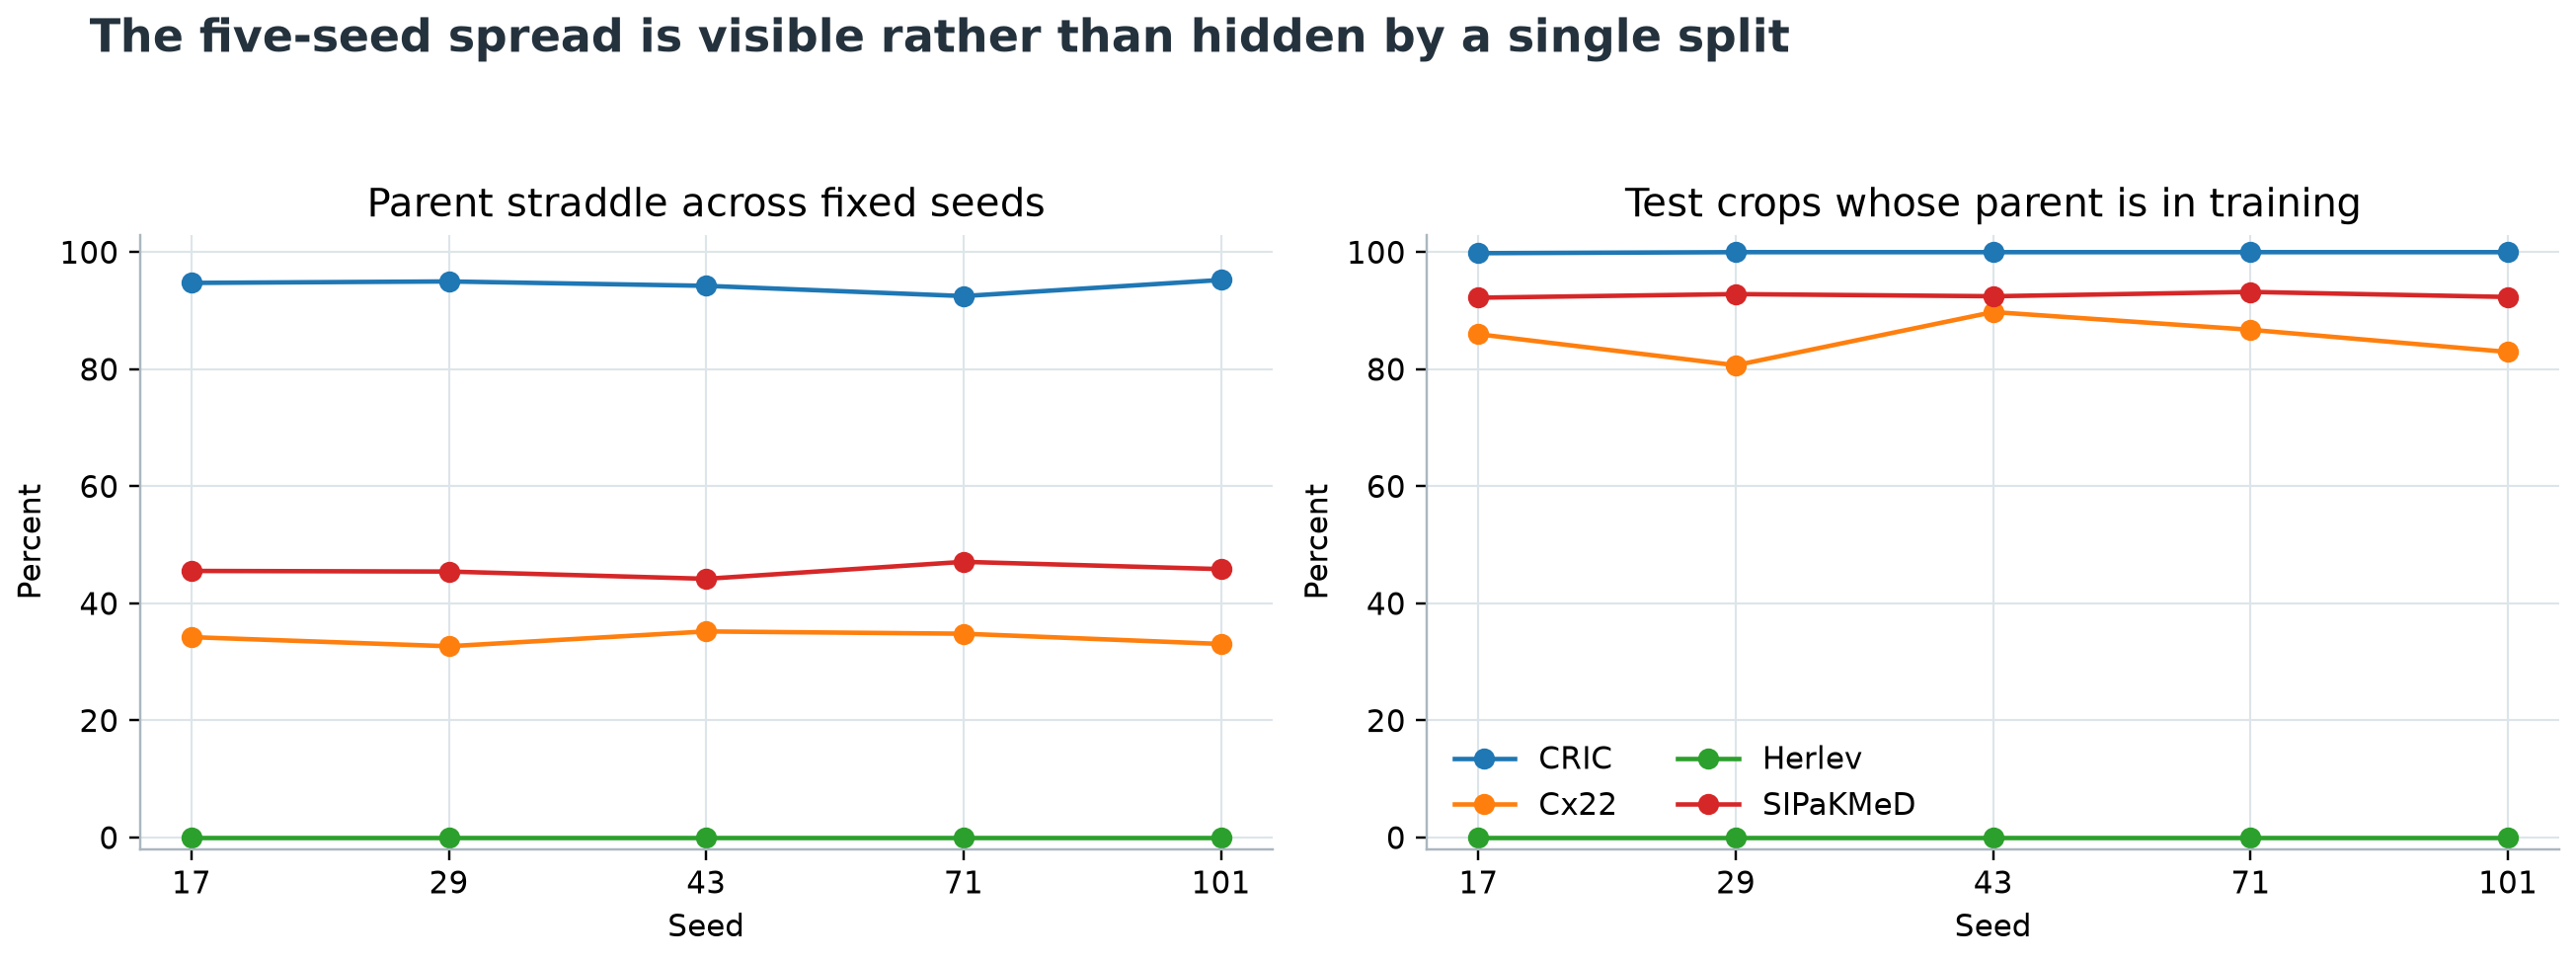
\includegraphics[width=\textwidth]{structural_seed_spread.png}
\caption{Seed-level structural results. Reporting the spread prevents one convenient split from defining the claim.}
\label{s1:fig:structural-seeds}
\end{figure}

\section{Interpretation}

CRIC is the most extreme because its parents emit 28.84 crops on average: essentially every random-split test cell has a source image in training. SIPaKMeD and Cx22 have lower parent multiplicity, yet 92.62\% and 85.23\% of their test observations respectively still have a training sibling. Herlev establishes implementation specificity: the same code returns zero when the data genuinely have one observation per parent.

The structural ordering P3 $\leq$ P2 $\leq$ P1 passes for all datasets. This statement concerns shared parents, not model scores. Later, the analogous model-score ordering fails for four of six SIPaKMeD classifiers; the two outcomes are logically compatible.
